\chapter{Results}\label{chap:results}
This chapter presents the results obtained from the modeling and simulation pipeline developed in this thesis. The 
evaluation focuses on two main aspects. First, the generated datasets are compared with the available reference data in 
order to assess their completeness. Second, the infrastructure elements extracted during the modeling process are analysed 
to evaluate the quality of the generated railway representation.

The results are presented separately for the macro-level and micro-level approaches when necessary. This distinction is 
important because the two models do not represent the railway network at the same level of detail. 

\section{Dataset Validation}
\subsection{Station Coverage}
Station coverage evaluates the number of stations detected and integrated into the generated datasets. This metric is 
important because stations are central elements in both modeling approaches. In the macro-level model, stations are the 
main nodes of the graph. In the micro-level model, stations are used to associate platforms and tracks with operational 
stopping points.

\begin{table}[H]
    \centering
    \begin{tabular}{lccc}
        \toprule
        Simulation Level & Generated Stations & Reference Stations & Coverage (\%) \cr
        \midrule
        Macro-Level & 559 & 559 & 100 \cr
        Micro-Level & 553 & 554 & 99.82 \cr
        \bottomrule
    \end{tabular}
    \caption{Station coverage for macro-level and micro-level simulations}\label{tab:station_coverage}
\end{table}

The results show that station coverage is very high for both modeling approaches. For the macro-level simulation, all 
559 stations present in the reference dataset are generated, corresponding to a coverage of 100.00\%. This indicates that, 
at the station-to-station level, the macro-level generation process is able to fully preserve the set of stations required 
for the generated network.

For the micro-level simulation, 553 stations are generated from a reference dataset containing 554 stations, corresponding 
to a coverage of 99.82\%. This result is also very strong, especially considering that the micro-level model requires a 
more detailed association between stations, platforms, and physical track infrastructure. The small difference between the 
reference and generated datasets may be explained by data inconsistencies, preprocessing filters, or the absence of a 
valid platform-track association for one station.

Overall, the station coverage results confirm that the generated datasets provide a reliable station basis for the rest of 
the modeling pipeline. The macro-level approach achieves complete station coverage, while the micro-level approach remains 
almost complete despite the additional infrastructure constraints introduced by the detailed model.

\subsection{Platform and Track Coverage}
The second part of the dataset validation concerns platform and track coverage. These elements are especially important 
for the micro-level model, where the objective is to represent the railway infrastructure in more detail. Platforms define 
where trains can stop inside stations, while tracks define the physical railway segments used for circulation.

\begin{table}[H]
    \centering
    \begin{tabular}{lccc}
        \toprule
        Category & Reference Data & Simulation Data & Coverage (\%) \cr
        \midrule
        Platforms & 1551 platforms & 1560 platforms & 99.42 \cr
        \midrule
        Tracks (Macro-Level) & 1385 tracks & 1560 tracks & 100 \cr
        \midrule
        Tracks (Micro-Level) & 25028 tracks & 26721 tracks & 106.59 \cr
        \bottomrule
    \end{tabular}
    \caption{Platform and track coverage for micro-level simulation}\label{tab:platform_track_coverage}
\end{table}

The platform coverage obtained for the micro-level model is also very high. The reference dataset contains 1560 platforms, 
while the generated dataset contains 1551 platforms, resulting in a coverage of 99.42\%. This shows that the platform 
detection and matching process is able to identify almost all platforms available in the reference data. However, it does 
not guarantee that the generated platforms are correctly positioned on the tracks, which is a separate aspect of the 
infrastructure modeling process.

Track coverage differs between the macro-level and micro-level models. In the macro-level simulation, the reference data 
contains 1385 station-to-station tracks and the generated dataset also contains 1385 tracks, giving a coverage of 100\%. 
This result is expected because the macro-level model directly represents connections between stations and does not 
attempt to reconstruct the detailed internal railway topology.

For the micro-level simulation, the generated dataset contains 26721 tracks, while the reference dataset contains 25068 
tracks. This corresponds to a coverage of 106.59\%. A value higher than 100\% does not necessarily indicate an error. It 
reflects the fact that the micro-level generation process may create more detailed or segmented track representations 
than those present in the reference dataset. In particular, a single reference track can be represented by multiple 
generated segments after preprocessing, switch detection, and track segmentation.

Overall, the platform and track coverage results show that the generated infrastructure is highly complete. However, the 
interpretation of track coverage must take into account the difference between reference tracks and simulation-ready 
SUMO edges. The generated micro-level network is not only a copy of the reference data, but a transformed representation 
adapted to routing and simulation constraints.

\section{Infrastructure Modeling Results}
After validating the general completeness of the datasets, the next step is to evaluate the results of the infrastructure 
modeling process. This part focuses on the railway elements that were extracted, transformed, or reconstructed during the 
implementation. The objective is to assess whether the generated infrastructure provides a coherent basis for railway 
simulation.

The infrastructure modeling results confirm the high level of coverage already observed in the dataset validation step. 
Stations are almost completely detected in both modeling approaches, and platforms are also recovered with a high success 
rate in the micro-level model. Switches require a more nuanced interpretation, because they are inferred from the 
generated railway topology rather than directly copied from the reference dataset.

\begin{table}[H]
    \centering
    \begin{tabular}{lccc}
        \toprule
        Category & Reference Data & Simulation Data & Detection (\%) \cr
        \midrule
        Stations (Macro-Level) & 559 & 559 & 100 \cr
        Stations (Micro-Level) & 554 & 553 & 99.82 \cr
        Platforms (Micro-Level) & 1560 & 1551 & 99.42 \cr
        Switches (Micro-Level) & 10379 & 12343 & 118.92 \cr
        \bottomrule
    \end{tabular}
    \caption{Detected stations, platforms and switches for macro-level and micro-level simulations}\label{tab:infrastructure_detection}
\end{table}

The detection percentage reaches 100.00\% for macro-level stations and 99.82\% for micro-level stations. Platform detection 
reaches 99.42\%, which confirms that most platforms could be matched to the generated infrastructure. These results are 
important because platforms are used as stopping locations for trains and as origin or destination points during trip 
generation.

Switch detection provides a different type of result. The reference data contains 10379 switches, while the generated 
micro-level infrastructure contains 12343 detected switches, corresponding to a coverage of 118.92\%. As with micro-level 
track coverage, this value above 100\% must be interpreted carefully. It does not simply mean that the model detects more 
correct switches than expected. Instead, it indicates that the algorithm identifies more candidate switch points than the 
number of switches available in the reference dataset.

\begin{figure}[H]
    \centering
    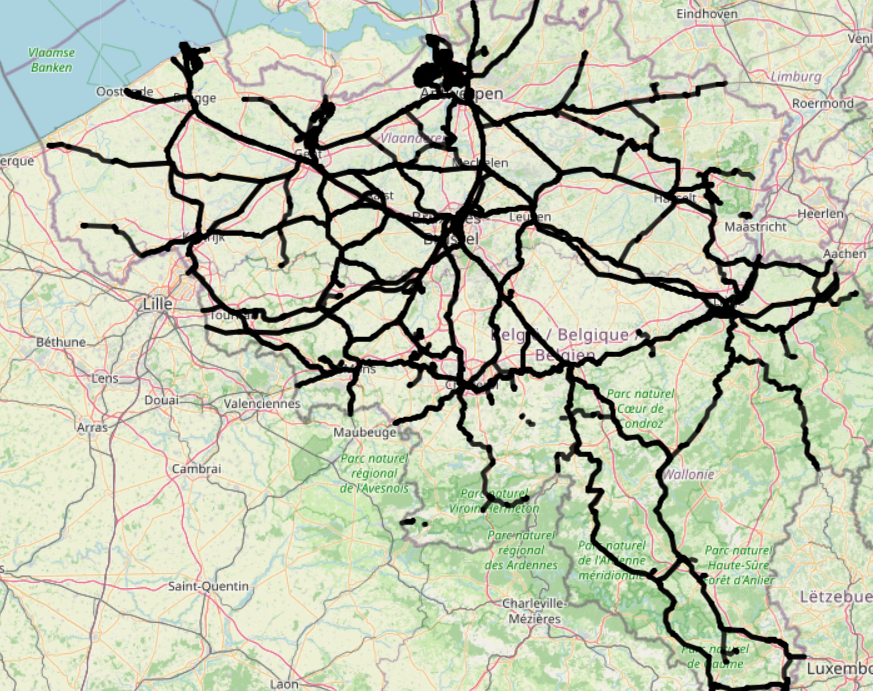
\includegraphics[width=0.6\textwidth]{chapters/images/switch_detection_before.png}
    \caption{Network before and after switch detection.}\label{fig:switch_detection_before}
\end{figure}

\begin{figure}[H]
    \centering
    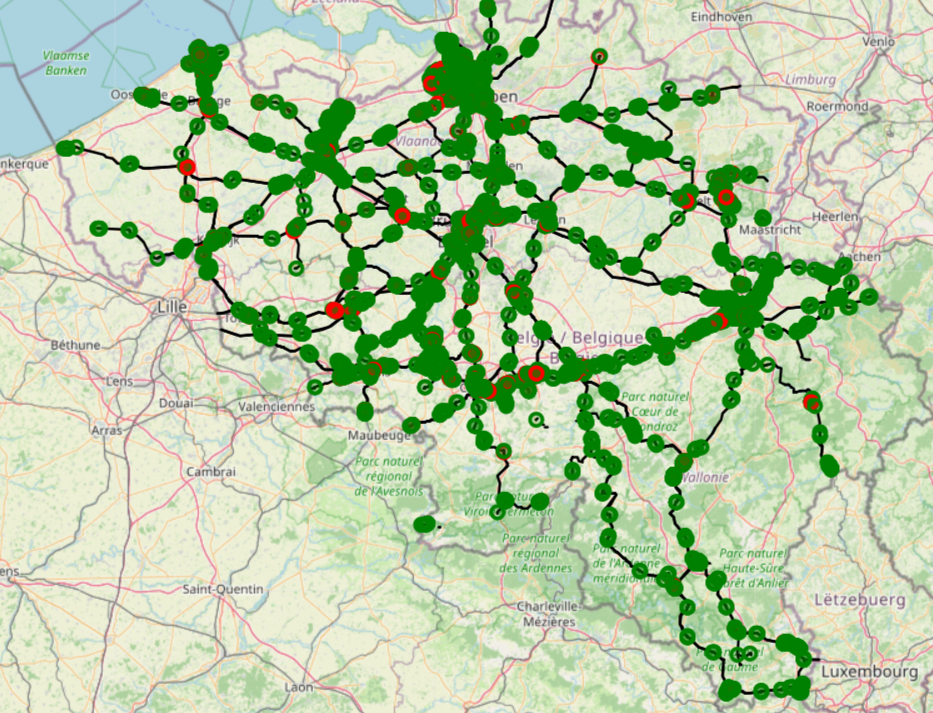
\includegraphics[width=0.6\textwidth]{chapters/images/switch_detection_after.png}
    \caption{Network before and after switch detection (Green dots represent detected switches with 3 connections and 
    Red dots represent detected switches with 4 or more connections)}\label{fig:switch_detection_after}
\end{figure}
This visual comparison makes it possible to understand how the algorithm enriches the infrastructure by identifying 
branching and merging points across the network.

This difference can be explained by the way switches are inferred from the railway topology. In the generated network, a 
switch is detected when a node connects more than two track segments and therefore behaves as a branching or merging point. 
However, this topological definition may identify some elements that are not classified as switches in the reference data. 
It may also split complex junctions into several smaller switch-like elements.

The visual comparison of the network before and after switch detection helps illustrate this effect. The switch detection 
process enriches the generated infrastructure by identifying relevant branching points and making the network more 
suitable for routing. In dense areas such as Bruxelles-Midi, the detected switches provide a much more detailed 
representation of the railway topology, but they also highlight the difficulty of matching generated topological elements 
exactly with reference infrastructure objects.

\begin{figure}[H]
    \centering
    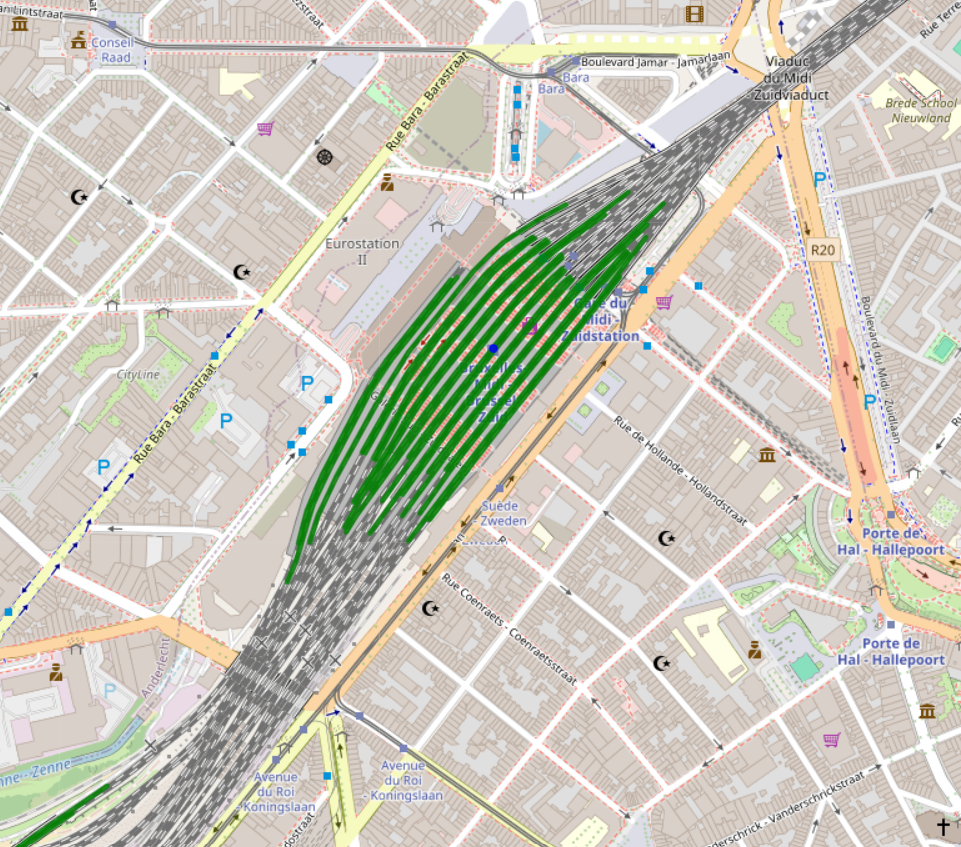
\includegraphics[width=0.6\textwidth]{chapters/images/platform_matching_result.png}
    \caption{Platform matching result on Bruxelles-Midi}\label{fig:platform_matching}
\end{figure}
This station is particularly relevant because it contains a dense set of tracks and platforms, making it a useful example 
for evaluating whether the platform matching algorithm can handle complex station environments.

\begin{figure}[H]
    \centering
    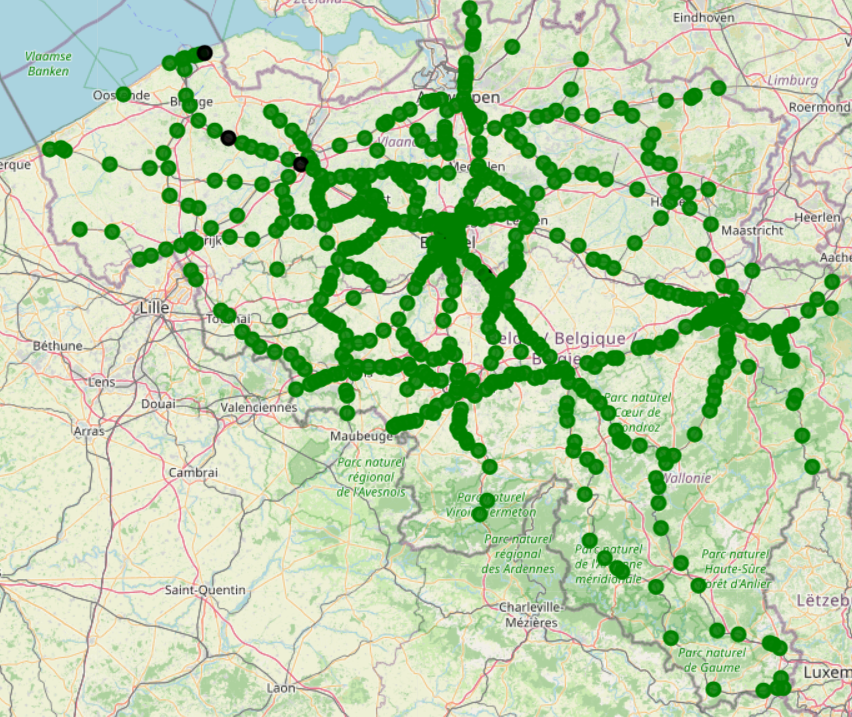
\includegraphics[width=0.6\textwidth]{chapters/images/platform_detection_quality.png}
    \caption{Platform matching quality map}\label{fig:platform_matching_quality}
\end{figure}


The platform matching figures further illustrate the quality of the generated infrastructure. They show how platforms are 
associated with the corresponding railway tracks and make it possible to visually inspect the quality of the matching 
process. This qualitative validation complements the numerical coverage metrics and helps identify local cases where the 
matching may be less accurate.

\begin{figure}[H]
    \centering
    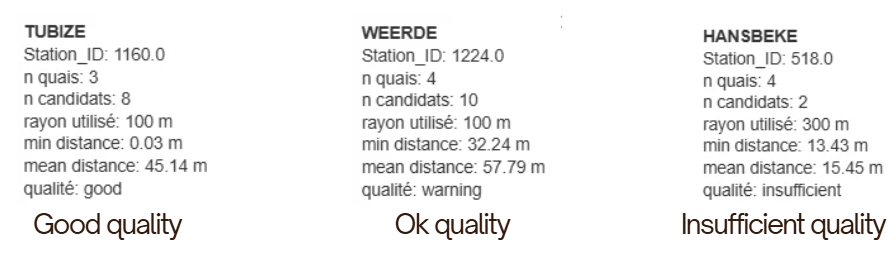
\includegraphics[width=0.6\textwidth]{chapters/images/platform_quality_example.png}
    \caption{Platform matching quality examples}\label{fig:platform_matching_examples}
\end{figure}
The platform matching quality is further illustrated by a qualitative comparison of several representative stations. As 
shown in Figure~\ref{fig:platform_matching_examples}, the matching process can produce different levels of quality 
depending on the local infrastructure configuration. For instance, Tubize is classified as a good-quality match, with a 
very small minimum distance between the detected platform and the candidate track, which suggests a reliable association. 
Weerde corresponds to an intermediate case, labelled as a warning, where the matching remains acceptable but presents a 
larger average distance, indicating a less precise association. By contrast, Hansbeke is classified as insufficient 
quality, showing that the algorithm may encounter difficulties in some local configurations, especially when the search 
radius is larger or when the number of candidate tracks does not allow a clear correspondence to be established.

\section{Simulation Results}


\section{Computational Performance}


\section{Discussion}